\documentclass[12pt, a4paper]{article}
\usepackage[utf8]{inputenc}
\usepackage{footnote}
\usepackage{hyperref}
\usepackage{fullpage}
\usepackage{amsmath}
\usepackage{pgfplots}
\usepackage{pgfplotstable}
\pgfplotsset{compat=1.8}
\usepackage{cleveref}
\usepackage{graphicx}
\usepackage{tocbibind}
\DeclareMathOperator*{\argmin}{\arg\!\min}
\newcommand{\colvec}[1]{\ensuremath{\begin{pmatrix}#1\end{pmatrix}}}

\begin{document}
\title{Bachelorarbeit\\ zur Erlangung des akademischen Grades\\ Bachelor of Science}
\author{Zachary Schellin\\376930}

\maketitle
\newpage
\tableofcontents
\newpage
\section{Introduction}
The Bhatnagar, Gross, Krook equation (BGK) is a kinetic collision model of ionized and neutral gases valid for rarefied as well as other pressure regimes \cite{BGK}. Generating data of such a flow field is essential for various industry and scientific applications[\textbf{REF}]. With the intention to reduce time and cost during the data generating process, experiments were substituted with computational fluid dynamics (CFD) computations. Consequently reduced-order models (ROMs) coupled to aforementioned computations were introduced to further the reduction of time and cost. The thriving field of artificial intelligence operates in model order reduction for data visualization/analysis since the 80's (Quelle?)  and has now surfaced in fluid mechanics. This thesis will cover the use of artificial intelligence for model order reduction in fluid mechanics.
\subsection{State of the art}
State of the art model reduction of dynamical systems is done via proper orthogonal decomposition (POD) which is an algorithm feeding on the idea of singular value decomposition (SVD)\cite{Franz}\cite{Kutz}. POD captures a low-rank representation on a linear manifold. So called POD modes, derived from SVD, describe the principle components of a problem which can be coupled within a Galerkin framework to produce an approximation of lower rank. 
\begin{equation}
	f(x)\approx \tilde{f}(x) \qquad\ \textrm{with}\qquad rk(f(x)) \gg rk(\tilde{f}(x))
\end{equation}
Bernard et al. use POD-Galerkin with an additional population of their snapshot database via optimal transport for the proposed BGK equation, bisecting computational run time (cost) in conjunction with an approximation error of ~ 1 \% \cite{Bernard}. Artificial intelligence in the form of autoencoders replacing the POD within a Galerkin framework is evaluated against the POD performance by Kookjin et al. for advection-dominated problems\cite{Carlberg} resulting in sub 0.1\% errors. An additional time inter- and extrapolation is evaluated. Using machine learning/ deep learning for reduced order modeling in CFD is a novel approach although "the idea of autoencoders has been part of the historical landscape of neural networks for decades"\cite[p.493]{Goodfellow}. Autoencoders, or more precisely learning internal representations by the delta rule (backpropagation) and the use of hidden units in a feed forward neural network architecture, premiered by Rumelhart et al. (1986) \cite{Rumelhart}.  Through so called hierarchical training Ballard et al.(1987) introduce a strategy to train auto autoassociative networks (nowadays referred to as autoencoders), in a reasonable time promoting further development despite computational limitations \cite{Ballard}. The so called bottleneck of autoencoders yields a non-smooth and entangled representation thus beeing uninterpretable by practitioners\cite{Rifai2011} leading to developements in this field. Rifai et al. introduce the contractive autoencoder (CAE) for classification tasks (2011), with the aim to extract robust features which are insensitive to input variations orthogonal to the low-dimensional non-linear manifold by adding a penalty on the frobenius norm of the instrinsic variables with respect to the input, surpassing other classification algorithms \cite{Rifai2011}. Subsequent development emerges with the manifold tangent classifier (MTC) \cite{Rifai_2011a}. A local chart for each datapoint is obtained hence characterizing the manifold  which in turn improves classification performance. On that basis a generative process for the CAE is developed. Through movements along the manifold with directions defined by the Jacobian of the bottleneck layer with respect to the input \begin{math}	\vec{x}_m=JJ^T \end{math}, sampling is realized \cite{rifai2012generative}. 
\subsection{Objective of this thesis}
Due to the non-linearity of transport problems in particular shock fronts, the construction of a robust ROM for those cases poses several challenges. Proper orthogonal decomposition (POD) and it's numerous variants like shifted-POD\cite{bibid}, POD-Galerkin\cite{bibid}, POD+I \cite{bibid} to name only a few of them, try to solve this problem by......
\subsection{Thesis outline}
\section{The BGK Equation}
\section{Reduced Order Algorithms}
\subsection{Data Sampling}
\subsection{POD}
The singular value decomposition of the input $X$ [REF to Section 1] gives the optimal low-rank approximation $\tilde{X}$ of $X$ \cref{Eg:eckard-young}[Eckard-Young]. \Cref{Fig:cumu_sing} shows the singular values (left) and the cumulative energy (right) derived from \cref{Eq:cumsum}:
\begin{equation}
S_N = \sum_{k=1}^{N}a_k \qquad\textrm{with a sequence} \qquad\{a_k\}_{k=1}^{n} 
\label{Eq:cumsum}
\end{equation}
\begin{equation}
\underset{\tilde{X}, s.t. rank(\tilde{X})=r}{\operatorname{argmin}} || X -\tilde{X} ||_F=\tilde{U}\tilde{\Sigma}\tilde{V}^*
\label{Eg:eckard-young}
\end{equation}
The first five singular values give an accurate approximation $\tilde{X}$ of $X$.  
As a means to evaluate the low-rank approximation of $X$ we will compare the density derived from \cref{Eq:dense}, computed from $X$ and $\tilde{X}$.
\begin{figure}[htb!]
	\centering
	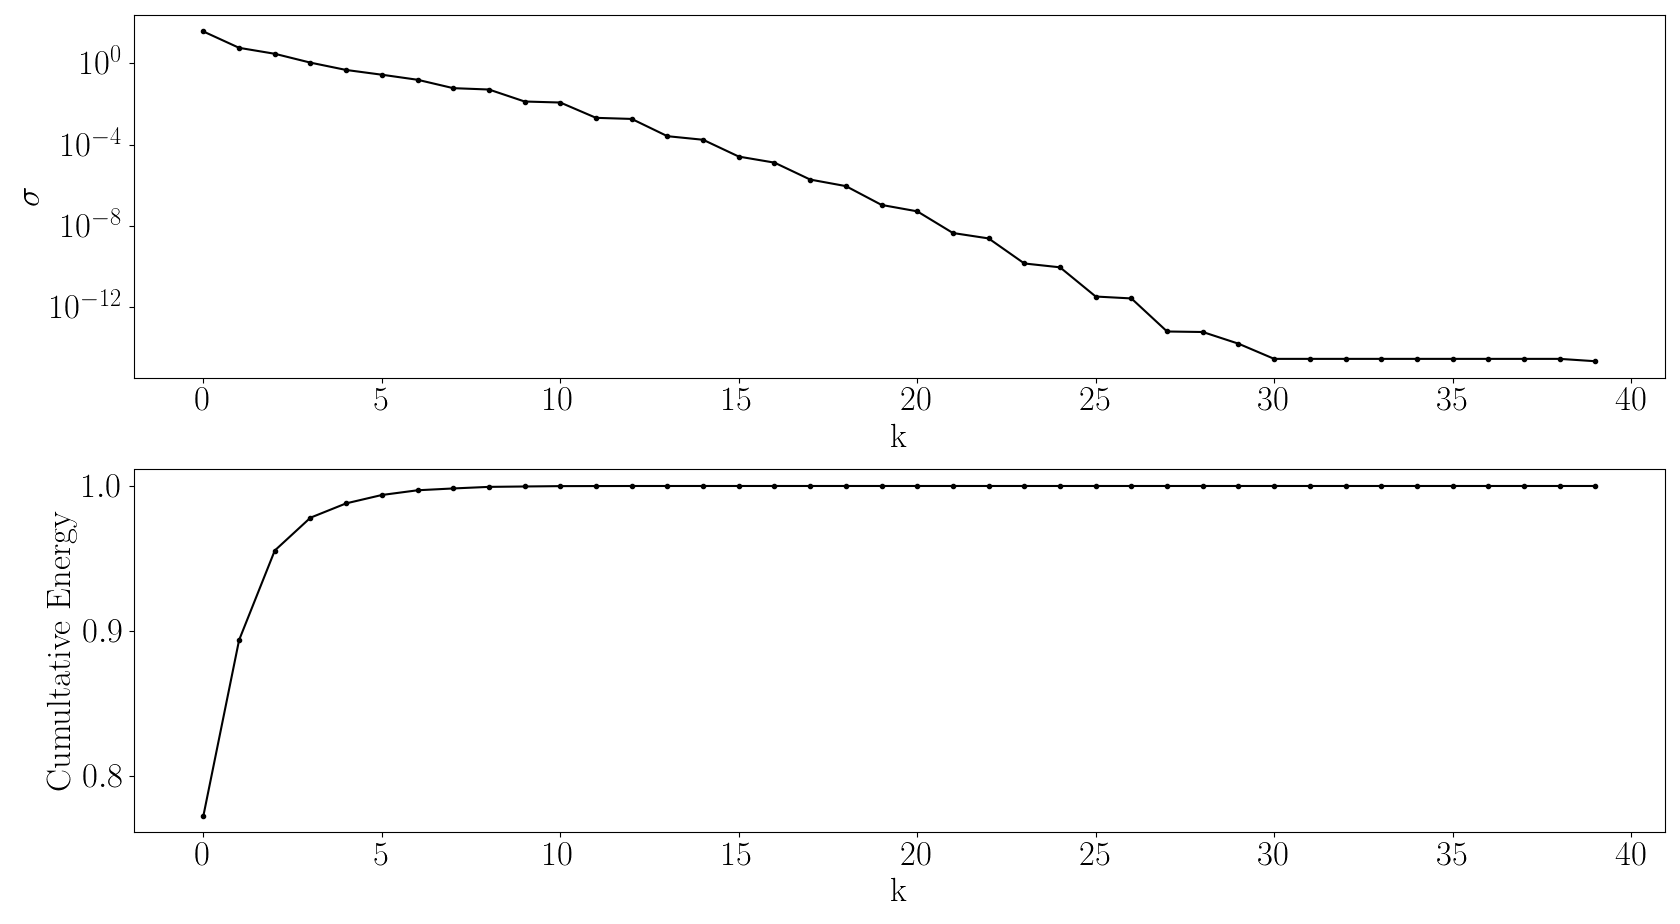
\includegraphics[width=\textwidth]{Figures/Cumultative_Singular_Values_kn001.png}
	\caption{Singular Values (left) and cumultative enrgy (right) over the number of singular values}
	\label{Fig:cumu_sing}
\end{figure}
\subsection{Autoencoders}
The same matrix as in POD is used as input data for the autoencoder:
\[S = \begin{bmatrix}
f(\xi_1,t_1,x_1)&\cdots &f(\xi_n,t_1,x_1) \\
f(\xi_1,t_1,x_2)&\cdots &f(\xi_n,t_1,x_2) \\
f(\xi_1,t_1,x_n)&\cdots &f(\xi_n,t_1,x_n)\\
f(\xi_1,t_2,x_1)&\cdots &f(\xi_n,t_2,x_1)\\
\vdots & \ddots & \vdots\\
f(\xi_1,t_n,x_n)&\cdots &f(\xi_n,t_n,x_n)
\end{bmatrix}\]
During training every 1000 epochs a sample against its prediction was printed in order to link the value of the L1-Loss to a prediction. Using this method a first verification of the model was achieved. Continuing the search for any possible shortage of the models performance, that this method could not cover, eg. samples lying between every 1000 sample, that the model was not able to reconstruct correctly, a second verification process is conducted. 
\section{Results and Latent Manifold Properties}
\subsection{Evaluation Methods}

\subsection{Results}
In a first attempt to construct the autoencoder, the architecture from \cite{Carlberg} is adopted. The architecture can be observed in:
\begin{center}
	\begin{tabular}{|c|c|c|c|c|}
		\hline
		Layer & Filter & Stride & Input Dim & Output Dim\\
		1	&	8	& 2x2	& 
	\end{tabular}
\end{center}

\subsection{Discussion and Outlook}
\bibliography{Bibliography}{}
\bibliographystyle{unsrt}
\end{document}
